% Options for packages loaded elsewhere
\PassOptionsToPackage{unicode}{hyperref}
\PassOptionsToPackage{hyphens}{url}
%
\documentclass[
]{article}
\title{Data Manipulation and Analysis in Stata}
\author{}
\date{\vspace{-2.5em}}

\usepackage{amsmath,amssymb}
\usepackage{lmodern}
\usepackage{iftex}
\ifPDFTeX
  \usepackage[T1]{fontenc}
  \usepackage[utf8]{inputenc}
  \usepackage{textcomp} % provide euro and other symbols
\else % if luatex or xetex
  \usepackage{unicode-math}
  \defaultfontfeatures{Scale=MatchLowercase}
  \defaultfontfeatures[\rmfamily]{Ligatures=TeX,Scale=1}
\fi
% Use upquote if available, for straight quotes in verbatim environments
\IfFileExists{upquote.sty}{\usepackage{upquote}}{}
\IfFileExists{microtype.sty}{% use microtype if available
  \usepackage[]{microtype}
  \UseMicrotypeSet[protrusion]{basicmath} % disable protrusion for tt fonts
}{}
\makeatletter
\@ifundefined{KOMAClassName}{% if non-KOMA class
  \IfFileExists{parskip.sty}{%
    \usepackage{parskip}
  }{% else
    \setlength{\parindent}{0pt}
    \setlength{\parskip}{6pt plus 2pt minus 1pt}}
}{% if KOMA class
  \KOMAoptions{parskip=half}}
\makeatother
\usepackage{xcolor}
\IfFileExists{xurl.sty}{\usepackage{xurl}}{} % add URL line breaks if available
\IfFileExists{bookmark.sty}{\usepackage{bookmark}}{\usepackage{hyperref}}
\hypersetup{
  pdftitle={Data Manipulation and Analysis in Stata},
  hidelinks,
  pdfcreator={LaTeX via pandoc}}
\urlstyle{same} % disable monospaced font for URLs
\usepackage[margin=1in]{geometry}
\usepackage{longtable,booktabs,array}
\usepackage{calc} % for calculating minipage widths
% Correct order of tables after \paragraph or \subparagraph
\usepackage{etoolbox}
\makeatletter
\patchcmd\longtable{\par}{\if@noskipsec\mbox{}\fi\par}{}{}
\makeatother
% Allow footnotes in longtable head/foot
\IfFileExists{footnotehyper.sty}{\usepackage{footnotehyper}}{\usepackage{footnote}}
\makesavenoteenv{longtable}
\usepackage{graphicx}
\makeatletter
\def\maxwidth{\ifdim\Gin@nat@width>\linewidth\linewidth\else\Gin@nat@width\fi}
\def\maxheight{\ifdim\Gin@nat@height>\textheight\textheight\else\Gin@nat@height\fi}
\makeatother
% Scale images if necessary, so that they will not overflow the page
% margins by default, and it is still possible to overwrite the defaults
% using explicit options in \includegraphics[width, height, ...]{}
\setkeys{Gin}{width=\maxwidth,height=\maxheight,keepaspectratio}
% Set default figure placement to htbp
\makeatletter
\def\fps@figure{htbp}
\makeatother
\setlength{\emergencystretch}{3em} % prevent overfull lines
\providecommand{\tightlist}{%
  \setlength{\itemsep}{0pt}\setlength{\parskip}{0pt}}
\setcounter{secnumdepth}{5}
\ifLuaTeX
  \usepackage{selnolig}  % disable illegal ligatures
\fi

\begin{document}
\maketitle

{
\setcounter{tocdepth}{2}
\tableofcontents
}
\hypertarget{introduction}{%
\section{Introduction}\label{introduction}}

Data manipulation is the process of cleaning, organising and preparing data in a way that makes it suitable for analysis. Most real-world datasets require some form of manipulation to facilitate the downstream analysis and this process is often repeated a number of times during the data analysis cycle. In this series you will learn how to manipulate raw data and prepare it for analysis and then to carry out simple analysis of yur data. The following topics are covered in the series:

\begin{itemize}
\item
  Learning to use multiple frames to work on data
\item
  Merging data sets, with and without frames
\item
  creating and dropping variables
\item
  using \texttt{preserve} and `restore
\item
  creating subsets of d
\item
  Reshaping data between long and wide form
\end{itemize}

There are ** sections to the tutorial, but each is quite short. There are few lengthy explanations. If you are not using this material in combination with a class, you will sometimes need to google for an explanation.

\emph{Last Updated: Feb 02, 2022 9:27 PM}

\hypertarget{acknowledgments}{%
\section{Acknowledgments}\label{acknowledgments}}

Content of this workshop is based on the following:

\begin{itemize}
\tightlist
\item
  \href{https://firecrest.io/tidydata_tutorial/index.html}{Data Manipulation in R}
\end{itemize}

Which is Altaf Ali's Excellent web based tutorial on using tidy data in R.

This work is licensed under a Creative Commons Attribution-ShareAlike 4.0 International License.

\hypertarget{getting-started}{%
\section{Getting Started}\label{getting-started}}

\hypertarget{prerequisites}{%
\subsection{Prerequisites}\label{prerequisites}}

Basic knowledge of working with data in Stata is essential. This course assumes that you're comfortable with reading datasets, working with do files, and navigating the Stata interface.

\hypertarget{software-requirements}{%
\subsection{Software Requirements}\label{software-requirements}}

\hypertarget{stata-release-17-or-later.}{%
\subsubsection{Stata Release 17 or later.}\label{stata-release-17-or-later.}}

Recent versions of Stata, 17 or later are required. You can check your version from the command line with:

\begin{verbatim}
version
\end{verbatim}

\hypertarget{some-using-stata-basics}{%
\section{Some using Stata basics}\label{some-using-stata-basics}}

\hypertarget{folders}{%
\subsection{Folders}\label{folders}}

I assume that you have a folder structure like

\begin{verbatim}
Project Folder
├── raw data
├── scripts
│   ├── cleanmydata.do
│   └── modelmydata.do
├── documentation
│   ├── PDFs
│   └── Word_docs
└──graphs
\end{verbatim}

Of course, other folder set-ups are possible, so be aware of your own as you follow the rest of this guide. The path to my main project folder,for example, is

\texttt{c:\textbackslash{}users\textbackslash{}jt\textbackslash{}Documents\textbackslash{}Projects\textbackslash{}StataWrangling}

\hypertarget{exercise}{%
\subsection{Exercise}\label{exercise}}

If you do not have a folder for your project (including for this training series project!), create one now with subfolders as above. You do not need to create the two do files in the scripts folder. You can do this in Stata if you know how or using your computers user interface.

\hypertarget{common-file-types}{%
\subsection{Common File types}\label{common-file-types}}

You will commonly encounter three types of file specific to Stata

\begin{itemize}
\tightlist
\item
  The .dta file which is Stata's proprietary data format;
\item
  The .do file which is Stata's scripting file type;
\item
  The .log file which is the file type recording session logs.
\end{itemize}

\hypertarget{the-do-file}{%
\section{The do file}\label{the-do-file}}

Do files are Stata's scripts. Simple programs made of text files of Stata commands.

Let's start off by creating a new do file:

\begin{verbatim}
doedit newdo.do
\end{verbatim}

You can also create a new do file editing session from the \textbf{Window} menu in Stata.

Clear everything to make sure there's nothing leftover in our environment

\begin{verbatim}
clear all
\end{verbatim}

\hypertarget{initialising-your-script}{%
\subsection{Initialising your script}\label{initialising-your-script}}

In a new data wrangling script you should

\begin{itemize}
\tightlist
\item
  start a log;
\item
  make sure you are in the correct project directory;
\item
  clear working memory.
\end{itemize}

So in your new do file add these lines:

\begin{verbatim}
capture log close
log using "MainProjectName $S_DATE.log", append
\end{verbatim}

or

\begin{verbatim}
cmdlog using "CommandsProjectName $S_DATE.log", append
\end{verbatim}

to log commands only and not output.

\hypertarget{exercise-1}{%
\subsection{Exercise}\label{exercise-1}}

Using your internet searching powers, find out why we wrote

\begin{verbatim}
capture log close
\end{verbatim}

at the start of the script, rather than just \texttt{log\ close}.

\hypertarget{which-directory}{%
\subsection{Which directory?}\label{which-directory}}

Next you should make sure you are in the correct directory.

To check which directory you are currently in type

\begin{verbatim}
pwd
\end{verbatim}

on the Stata console.

Normally for a data wrangling script, this will be the \texttt{raw\ data} directory for the project by adding a line like

\begin{verbatim}
cd c:\users\jt\Documents\Projects\StataWrangling\raw data\
\end{verbatim}

(you must alter this to point at your folder) and then the line

\begin{verbatim}
clear all
\end{verbatim}

to start with a clear workspace.

\hypertarget{exercise-2}{%
\subsection{Exercise}\label{exercise-2}}

Close the log file or log files you have created and outside of Stata find the files and view the content.

\hypertarget{dataset}{%
\section{Dataset}\label{dataset}}

We're using a dataset of examination results from thirty school students.

These data are in in csv format: comma seperated values. Each case or observation is a row with variables in rows seperated by commas.

The data look something like this:

\begin{longtable}[]{@{}lrrrrr@{}}
\toprule
surname & sex & class & maths & english & history \\
\midrule
\endhead
ADAMS & 2 & 1 & 55 & 63 & 65 \\
ALI & 2 & 1 & 52 & 46 & 35 \\
BAGAL & 1 & 3 & 51 & 58 & 55 \\
BENJAMIN & 1 & 2 & 59 & 70 & 68 \\
BLAKEMORE & 2 & 2 & 56 & 38 & 40 \\
\bottomrule
\end{longtable}

The Stata \texttt{use} command reads in data from Stata format files. Read the main data file by adding this command to your do file:

\begin{verbatim}
use https://www.ucl.ac.uk/~ccaajim/results
\end{verbatim}

When you first read a datafile, you should always

\begin{itemize}
\tightlist
\item
  \texttt{describe} the data;
\item
  check the codebook.
\end{itemize}

You can do this for the complete set of variables for simple cases, but you may wish to be selective when you have a lot of variables.

\hypertarget{data-types}{%
\subsection{Data Types}\label{data-types}}

The examination data is quite simple. In your do file add

\begin{verbatim}
describe
codebook
\end{verbatim}

And run the do file. This first command produces

\begin{figure}
\centering
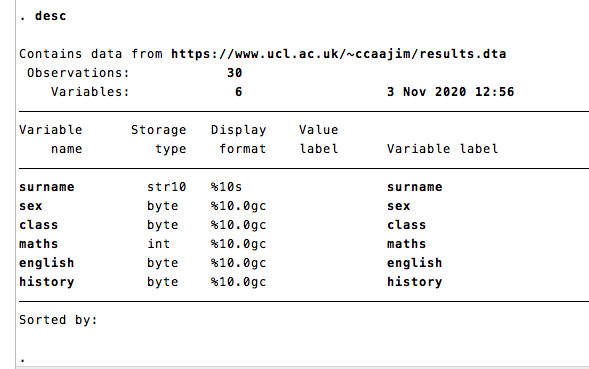
\includegraphics{./images/describeoutput1.png}
\caption{The main Stata results screen showing the output of desc}
\end{figure}

\hypertarget{interpretation-of-describe-output}{%
\subsection{\texorpdfstring{Interpretation of \texttt{describe} output}{Interpretation of describe output}}\label{interpretation-of-describe-output}}

This output shows first how many observations there are in your data and how many variables. The table that follows includes some detail about each variable:

\textbf{Storage type} There are two basic data types in Stata: \emph{numeric} and \emph{string} data. String data has two subtypes: strL (L for long) variables can store phenominal amounts of character data (2 billion) and str\# (where \# is a number) and have a limit on length of 2045 characters. Numeric data is of one of five types:

\begin{longtable}[]{@{}lll@{}}
\toprule
type & precision & range \\
\midrule
\endhead
byte & integer & -127 to 100 \\
int & integer & -32,767 and 32,740 \\
long & integer & -2,147,483,647 and 2,147,483,620 \\
float & real & 8 digits of accuracy \\
double & real & 16 digits of accuracy \\
\bottomrule
\end{longtable}

Format types are associated with variables - each has a default, which determines how values are displayed, so that regardless of the precision of the type, the number of decimal places and the width in number of characters to be displayed can be fixed. So a format type \texttt{\%9.0g} is a left justified number of maximum 9 characters in width and with specific decimal precision (although in this case zero means 'just as many as can be displayed for this width).

\hypertarget{interpretation-of-codebook}{%
\subsection{Interpretation of codebook}\label{interpretation-of-codebook}}

The output of \texttt{codebook} shows you the data type of the variables; the range and the numeric unit of measure; the number of unique values in the data; the number of values missing; the mean value for continuous variables; the standard deviation; the percentile values for the 10\%, 25\%, 50\%, 75\%, 90\% points.

The value of output from \texttt{codebook} is enhanced if you have taken care to label variables and values.

\hypertarget{exercise-3}{%
\subsection{Exercise}\label{exercise-3}}

What are the types and formats of the variables \texttt{maths}, \texttt{english}, \texttt{history}? Why is \texttt{maths} different?

\hypertarget{listing-and-sorting}{%
\section{Listing and Sorting}\label{listing-and-sorting}}

\hypertarget{listing-cases}{%
\subsection{Listing cases}\label{listing-cases}}

To list data in the main results window you use the list command. If you type

\begin{verbatim}
list maths english
\end{verbatim}

on the console, Stata will respond by list all observations for those variables. If you don't specify variables Stata use all the variables.

\hypertarget{exercise-4}{%
\subsection{Exercise}\label{exercise-4}}

Type following line on the console

\begin{verbatim}
list maths class in 1/6
\end{verbatim}

How would you describe the effect of the modifier \texttt{in\ 1/6}

\hypertarget{sorting}{%
\subsection{Sorting}\label{sorting}}

\hypertarget{detecting-and-correcting}{%
\section{Detecting and correcting}\label{detecting-and-correcting}}

In the data as you find it, there is an anomalous maths score. We can find this my simple inspection of the data because we have a small data set and few variables. If we had a larger data set with many variables this would be much more difficult. We will write some code to help us in the detection of variables.

In Stata we can use programming functions that return values. Many functions return vales \textbf{true} or \textbf{false}. There is a function \textbf{inrange(variable, min, max)} that returns true if \emph{variable} is less greater than \emph{min} and less than \emph{max}. We negate functions with the operator meaning \textbf{not} - \emph{!}.

\hypertarget{exercise-5}{%
\subsection{Exercise}\label{exercise-5}}

In your script add the following lines:

\begin{verbatim}
gen anomaly = 0
replace anomaly = 1 if !inrange(maths,0,50)
\end{verbatim}

Are after you run these lines, are there any anomalous cases in your dataset? How many?

The Stata symbol for or is \textbf{\textbar{}} sometimes called bar or pipe.

Alter the second line above so that it checks not only \texttt{maths} but the \texttt{english}, \texttt{history} and \texttt{avxm} variables as well.

\hypertarget{replacing-values}{%
\subsection{Replacing values}\label{replacing-values}}

In the data for this tutorial, there is one score in \texttt{maths} that is clearly out of range. In this case we need to replace the \texttt{maths} score for the student with \texttt{surname} DENCIK. So we can do that on the Stata command line with a replace command. Preserve the current state of your data with \texttt{preserve} and then type this command on the console:

\begin{verbatim}
replace maths = 57 if surname == "DENCIK"
\end{verbatim}

When you have inspected the data to ensure the correction has been made, \texttt{restore} the snapshot from before correction.

\hypertarget{exercise-6}{%
\subsection{Exercise}\label{exercise-6}}

Correct the anomalous \texttt{maths} score, but do not base the replacement on the \texttt{surname} variable, rather use only the \texttt{maths} values.

\hypertarget{selecting-variables-in-operations}{%
\section{Selecting variables in operations}\label{selecting-variables-in-operations}}

We will use the command \texttt{list} which displays rows of variable values to illustrate the selection of variables.

With most commands, variables can be included in the \emph{varlist} that follows a command name. So on the command line we can type

\begin{verbatim}
list maths english history
\end{verbatim}

which displays all the values for those three variables. Much of the time this is the only selection of variables you need.

But, there are times when you wish to select a subset of variables for manipulation perhaps for a series of operations. In this case we can use \texttt{preserve} and \texttt{restore}.

The command \texttt{preserve} takes a snapshot of a data set. If we then manipulate or modify the data, we can return to the snapshot state with the command \texttt{restore}. You can now use \texttt{drop\ varlist} to remove variables from the workspace or \texttt{keep\ varlist} to specify variables to be kept in the workspace.

Stata has a built in \emph{macro} (Stata speak for a script variable) named \textbf{\_all} that contains all the variable names currently in memory.

\hypertarget{exercise-7}{%
\subsection{Exercise}\label{exercise-7}}

Add the following lines to your script

\begin{verbatim}
    preserve
    keep maths english history
    summarize _all
    restore
    
\end{verbatim}

What is the effect of these lines?

How many variables are in working memory after the \texttt{keep} command? How many variables are in working memory after the \texttt{restore} command?

\hypertarget{the-uses-of-_all}{%
\subsection{The uses of \_all}\label{the-uses-of-_all}}

The \texttt{\textbackslash{}\_all} macro is obviously useful. but as the exercise shows, it can be more useful combined with \texttt{drop} and \texttt{keep}. The command \texttt{drop\ varlist} removes variables from the workspace, while \texttt{keep\ varlist} drops all but the named variables.

So, if we want to produce summary statistics for all continuous variables in our data, we can use \texttt{keep} followed by the list of names and then calculate the summaries.

\hypertarget{exercise-8}{%
\subsection{Exercise}\label{exercise-8}}

Add the following lines to your script

\begin{verbatim}
preserve
keep maths english history
tabstat _all, statistics(mean sd var kurt skew)
restore
\end{verbatim}

Answer these questions:

\begin{enumerate}
\def\labelenumi{\arabic{enumi}.}
\tightlist
\item
  What is the Skewness of the \textbf{mathematics} scores?
\item
  Which scores show more variability, \textbf{English} or \textbf{History}?
\item
  Which subject has the lowest mean score?
\end{enumerate}

\hypertarget{creating-a-custom-variable-list}{%
\subsection{Creating a custom variable list}\label{creating-a-custom-variable-list}}

Since many commands take a list of variables to operate on, it can be useful to create a specific list of variables that you can easily refer to repeatedly. We will do this with a Stata \texttt{global} macro.

Add the following lines to your script

\begin{verbatim}
global conts maths english history
summarize $conts
\end{verbatim}

Since in this case we don't drop any variables, we don't \texttt{preserve} and \texttt{restore}.

\hypertarget{labelling}{%
\section{Labelling}\label{labelling}}

\hypertarget{variables}{%
\subsection{Variables}\label{variables}}

Variable names are not always very human friendly. It is useful therefor to be able to attach a \textbf{label} to a variable, especially for using in output such as graphs.

Add the following line of code to your script

\begin{verbatim}
label variable sex "Gender"
\end{verbatim}

now use the \texttt{table} command to view a table of frequencies of the \texttt{sex} variable. What has been the effect of your line of code?

\hypertarget{exercise-9}{%
\subsection{Exercise}\label{exercise-9}}

Create appropriate labels for the variables in your dataset.

\hypertarget{values}{%
\subsection{Values}\label{values}}

When we code some categorical variables, we will often use a \emph{code} to represent the different possible values. for example, we might code eyecolour as

\begin{longtable}[]{@{}ll@{}}
\toprule
Code & Meaning \\
\midrule
\endhead
1 & Brown \\
2 & Blue \\
3 & Grey \\
4 & Green \\
5 & Other \\
\bottomrule
\end{longtable}

The use of numeric codes is very convenient in many circumstances, but it is not very human friendly. We would also like to put more meaningful labels for the values on output such as tables and graphs. To do this we create a \textbf{label set} and apply it to the variable values.

The label set is a list of codes and meanings create by a command like

\begin{verbatim}
label define eyecolourlabels 1 "Brown" 2 "Blue" 3 "Grey" 4 "Green" 5 "Other"
\end{verbatim}

We apply the labels to values of a variable \texttt{eyecolour} with a command like

\begin{verbatim}
label values eyecolour eyecolourlabels
\end{verbatim}

\hypertarget{exercise-10}{%
\subsection{Exercise}\label{exercise-10}}

Create an appropriate label set for the variable \texttt{sex} in your data set and apply it to the values of \texttt{sex}. Use the \texttt{list} command to check the results. What do you see?

\hypertarget{some-exploratory-analysis}{%
\section{Some exploratory analysis}\label{some-exploratory-analysis}}

Before embarking on the systematic modelling and testing of data, you may wish to explore its broad outline. There are several useful Stata procedures for this task:

\begin{itemize}
\item
  simple visualisatons:

  \begin{itemize}
  \tightlist
  \item
    box plots;
  \item
    histograms;
  \item
    bar charts;
  \end{itemize}
\item
  summary statistics;
\item
  tables.
\end{itemize}

\hypertarget{simple-visualisations}{%
\subsection{Simple visualisations}\label{simple-visualisations}}

For continuous numeric data you can create box plots and histograms. In your do file add the line

\begin{verbatim}
hist maths
\end{verbatim}

You might like to create graphs for a list of variables. First create a macro containing the variable names, then create the histograms. Try the following lines

\begin{verbatim}
global conts maths english history
hist $conts
\end{verbatim}

Unfortunately, as soon as Stata creates a new graph, the currently open graph window is destroyed. We can avoid this outcome by creating and exporting the histograns in a program loop. Add the following lines to your script

\begin{verbatim}
foreach var in $conts {
    hist `var'
    graph export `var'.png
}
\end{verbatim}

Once this loop terminates, you can look in your current directory to find the exported graphs.

You can dig deeper into your data by grouping values by any factor (categorical) variables, for example

\begin{verbatim}
graph box $conts, over(sex)
\end{verbatim}

\hypertarget{exercise-11}{%
\subsection{Exercise}\label{exercise-11}}

Create histograms for the \texttt{english} and\texttt{history} data. How similar or dissimilar do you think these data are?

Create box plots of \texttt{maths} for each level of\texttt{sex}. How do you think the male and female maths scores compare?

\hypertarget{summary-statistics}{%
\subsection{Summary statistics}\label{summary-statistics}}

Quick summary statistics for continuous numeric variables can be calculated with the \texttt{summarize} command. Try the command

\begin{verbatim}
summarize maths
\end{verbatim}

\end{document}
